\chapter{Congruence}

Look at this picture of two geometric figures.

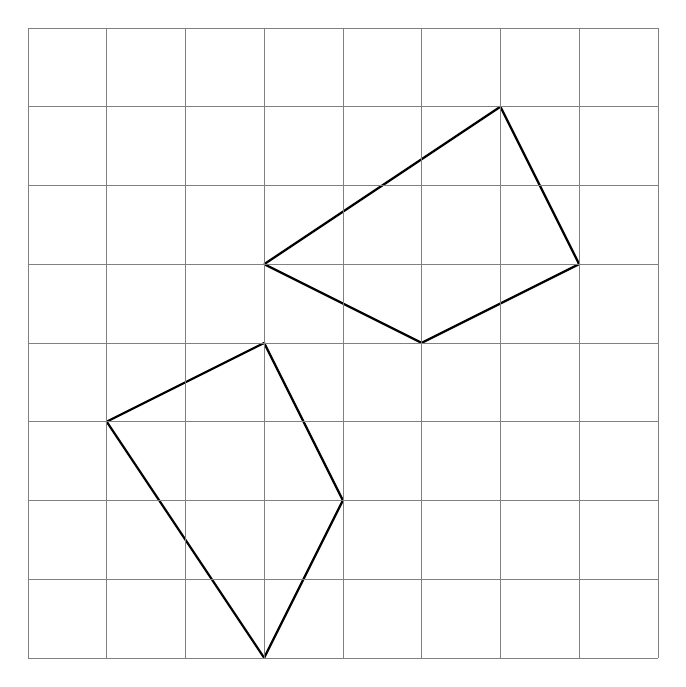
\begin{tikzpicture}
 
  	\draw [thick] (-1,-4) --  (0, -2);
	\draw [thick] (0,-2) --  (-1, 0) ;
	\draw [thick] (-1,0) --  (-3, -1); 
	\draw [thick] (-3,-1) --  (-1, -4);
	
	\draw [thick] (-1,1) --  (1, 0);
	\draw [thick] (1,0) --  (3, 1) ;
	\draw [thick] (3,1) --  (2, 3); 
	\draw [thick] (2,3) --  (-1, 1);

  \draw[help lines, step = 1cm] (-4, -4) grid (4, 4);
 
\end{tikzpicture}

They are the same shape, right? If you cut one out with scissors, it
would lay perfectly on top of the other. In geometry, we say they are
\emph{congruent}.

What is the official definition of ``congruent''? Two geometric
figures are congruent if you can transform one into the other using
only rigid transformations.  So, what are rigid transformations?

A transformation is \emph{Rigid} if it doesn't change the distances
between the points or the measure of the angles between the lines they
form. These are all rigid transformations:
\begin{itemize}
\item Translations
\item Rotations
\item Reflection 
\end{itemize}

If you once again imagine cutting one figure out with scissors and trying to match it with the second:
\begin{itemize}
\item Translations - sliding the cutout left and right and up and down
\item Rotations	- rotating the cutout clockwise and counterclockwise
\item Reflection - flipping the piece of paper over
\end{itemize}

A transformation is rigid if and only if it is some combination of translations, rotations, and reflections.

\section{Triangle Congruency}

If the sides of two triangles have the same length, the triangles must be congruent:

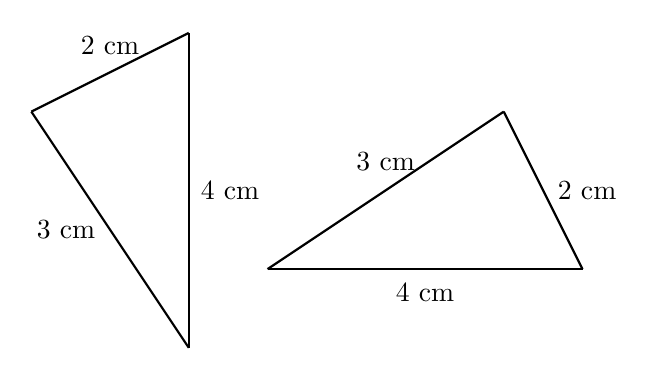
\begin{tikzpicture} 
  	\draw [thick] (-2,0) -- node[outer sep = 1pt, right]{4 cm}  (-2, 4) ;
	\draw [thick] (-2,4) --  node[outer sep = 3pt, above]{2 cm} (-4, 3); 
	\draw [thick] (-4,3) --  node[outer sep = 2pt, left]{3 cm} (-2, 0);
	
	\draw [thick] (-1,1) --  node[outer sep = 2pt, below]{4 cm}  (3, 1) ;
	\draw [thick] (3,1) --  node[outer sep = 2pt, right]{2 cm} (2, 3); 
	\draw [thick] (2,3) --  node[outer sep = 4pt, above]{3 cm} (-1, 1);
\end{tikzpicture}

To be precise, the Side-Side-Side Congruency Test says that two triangles are
congruent if three sides in one triangle are the same length as the
corresponding sides in the other. We usually refer to this as the SSS test.

